\documentclass[a4paper,10pt]{beamer}
\usetheme{metropolis}


\usepackage[T1]{fontenc}	%Correct accented characters and copy paste them, also not unexpected results with some characters like pipe
\usepackage[utf8]{inputenc}
\usepackage[spanish, es-tabla,es-noindentfirst]{babel}		%http://www.tex-tipografia.com/spanishopt.html
\spanishdecimal{.}
\usepackage[document]{ragged2e}	%centering
%\usepackage{listings}			%highlight code
	%\lstset{breaklines}			%line wrap for listings
	%\newcommand{\lstlistinginput}{\lstinputlisting}		%alias
%\usepackage{courier}		%listings better font
\usepackage{multicol}
\usepackage{multirow}
\usepackage{hyperref}
\usepackage{enumitem}
\usepackage[labelformat=empty]{caption}
\usepackage{graphicx}		%Introduces the \includegraphics command, which is needed for inserting figures
%\usepackage[sorting=none]{biblatex}
	%\addbibresource{bib.bib}
\usepackage{pgf-pie}
\usepackage[official]{eurosym}
\usepackage{tikz}
\usepackage{forest}
\usetikzlibrary{arrows,shapes,positioning,shadows,trees,decorations.markings}
\def\checkmark{\tikz\fill[scale=0.4,color=black!30!green](0,.35) -- (.25,0) -- (1,.7) -- (.25,.15) -- cycle;} 
\def\crossmark{\textcolor{black!10!red}{X\ }}


%\setbeamertemplate{bibliography item}{\insertbiblabel}				%beamber numbered bibliography for bibtex and biblatex

\setbeamerfont{section in toc}{series=\bfseries}


%%%%%%%%%%%%%%%%%%%%%%%%%		MORE	ALIASES		%%%%%%%%%%%%%%%%%%%%%%%%%

\newcommand{\lineh}{\rule{\textwidth}{1pt}\hfill\break}
\newcommand{\linej}{\hfill\break}









\begin{document}


\begin{frame}[fragile]
	\linej
	\linej
	\linej
	\large
	\centerline{\textbf{Mejoras en IDS: añadiendo funcionalidad a Wazuh}}
	\normalsize
	\linej
	\linej
	\centerline{github.com/andresgomezvidal/tfg\_memoria}
	\linej
	\linej
	\begin{multicols}{2}
	\textbf{Autor:}
	\linej
		Andrés Santiago Gómez Vidal
	\linej
	\columnbreak
	\linej
	\textbf{Tutores:}
	\linej
		Purificación Cariñena Amigo
	\linej
		Andrés Tarascó Acuña
	\end{multicols}

%Hablar:
	%Buenos días, soy Andrés Gómez y voy a proceder con la defensa de mi TFG: "Mejoras en IDS: añadiendo funcionalidad a Wazuh".
	%Mis tutores fueron Purificación Cariñena Amigo (de la universidad) y Andrés Tarascó Acuña (de la empresa Tarlogic, de la que no formo parte).
\end{frame}


\section{Introducción}
\begin{frame}[fragile]
	\frametitle{Motivación}

	\begin{itemize}
		\item La seguridad informática avanza continuamente. %Dificultada para asegurar que un sistema sea completamente seguro. Tanto por vulnerabilidades conocidas como no.
		\item Las medidas de prevención no son suficientes. %Como los Cortafuegos
	\end{itemize}
\end{frame}

\begin{frame}[fragile]
	\frametitle{Diferencias principales}
	\resizebox{\textwidth}{!}{%
	\begin{tabular}{|c|c|c|} \hline
	\centering
		& \textbf{IDS} & \textbf{Antivirus tradicional} \\ \hline
		\textbf{Recopilación} & Información masiva de multiples sistemas& Información local\\ \hline
		\textbf{Análisis} & Eventos y flujos de datos & Programas y archivos \\ \hline
		\textbf{Detección} & Objetivos & Técnicas \\ \hline
	\end{tabular}}
\end{frame}

\begin{frame}[fragile]
	\frametitle{Objetivos}

	\begin{itemize}
		\item Detectar posibles intrusiones en sistemas. %Para mitigarlas. Con un IDS (explicar significado IDS). Concretamente usamos la detección con patrones en vez de con comportamiento porque se nos iba del alcance.
		\item Crear la configuración para detectar ciertas amenazas reales. %de las más importantes actualmente. En vez de crear un IDS de cero usamos uno existente y simplemente añadimos la configuración para poder detectar lo que nos interesa, aumentando su funcionalidad a efectos prácticos. Explicar que la idea inicial incluía desarrollar código para el propio IDS si hubiera tiempo.
	\end{itemize}
\end{frame}

\begin{frame}[fragile]
	\frametitle{¿Qué es OSSEC?}

	\begin{itemize}
		%\item IDS empleado en el proyecto. %en vez de crear uno de cero
		\item Escalable con agentes. %como mínimo hace falta un servidor
		\item Basado en reglas y alertas. %recopila información con los agentes, que se procesa contra reglas, pudiendo generar alertas
		\item Compatible con muchos sistemas operativos: Windows, Mac OS, GNU/Linux, etc.
		\item Integrable con otras herramientas: Docker, Puppet, Ansible, OSQuery, VirusTotal, Suricata, OwlH, Bro, etc.
	\end{itemize}
\end{frame}

\begin{frame}[fragile]
	\frametitle{¿Qué es Wazuh?}

	\begin{figure}[H]
		\centering
		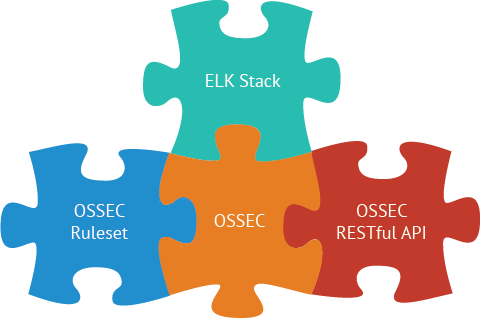
\includegraphics[width=.7\textwidth]{../figuras/wazuh_stack.png}
	\end{figure}

%Hablar:
	%Es una versión de OSSEC con añadidos para que sea más simple de implantar en los sistemas.
	%El stack ELK se refiere a las herramientas de procesado de datos: ElasticSearch, Logstash y Kibana.
	%Básicamente está pensado para integrarse en un sistema y proveer detección para situaciones normales sin configuración extra.
	%Por ejemplo Wazuh permite analizar alertas a través del navegador.
\end{frame}

\begin{frame}[fragile]
	\frametitle{Procesamiento de reglas}

	\begin{figure}[H]
		\centering
		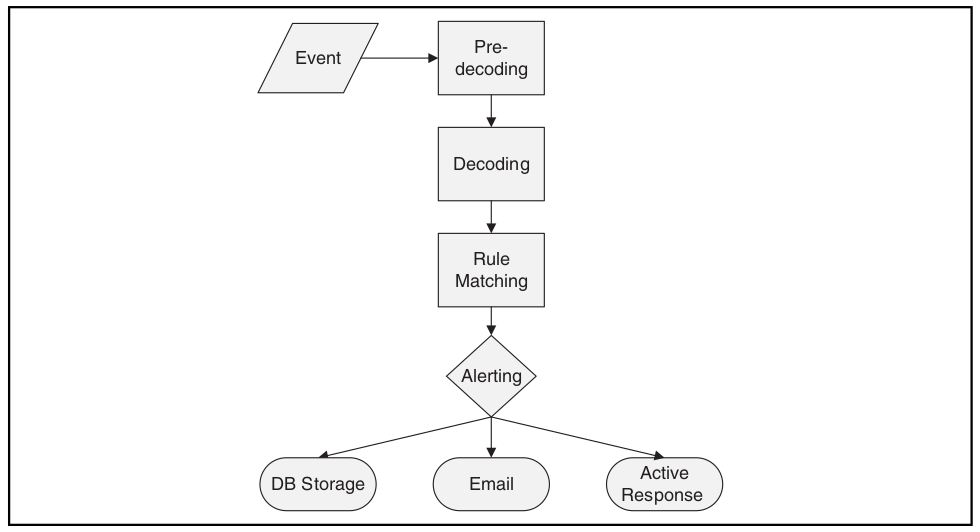
\includegraphics[width=\textwidth]{../figuras/Event_Flow.png}
	\end{figure}

%Hablar:
	%Para cada evento recibido de los agentes:
	%Primero se decodifica: se divide en campos
	%Luego se comprueba si se corresponde con alguna regla.
	%En cuyo caso se pude lanzar una alerta.
	%Además se puede almacenar información en una base de datos, enviar un email o ejecutar un script (respuesta activa).
		%La respuesta activa abre muchas posibilidades de intervención automática. Por desgracia actualmente no es casi configurable.
\end{frame}

\begin{frame}[fragile]
	\frametitle{Procesamiento de reglas}

	\begin{itemize}
		\item Atómicas y compuestas.
		\item Estructura padre-hijo.
		\item Expresiones regulares y variables.
		\item Pueden no generar ninguna alerta.
	\end{itemize}

%Hablar:
	%Hay 2 tipos de reglas: atómicas y compuestas. Las atómicas son independientes unas de otras y las compuestas necesitan que se cumplan varias atómicas en un intervalo de tiempo.
	%Las reglas se procesan por un sistema de padre-hijo. Si se cumple el padre se van comprobando los hijos hasta que se cumpla uno. Así sucesivamente hasta el final, sin volver nunca atrás.
	%Se puede conseguir cierta abstracción con expresiones regulares y variables, pero solamente si se conocen al iniciar el servicio.
	%Por eso y porque pueden no generar ninguna alerta se pueden crear muchas combinaciones de reglas que son procesadas eficientemente, a coste de que sean más complicadas de crear para el administrador.
\end{frame}


\section{Gestión del proyecto}
\begin{frame}[fragile]
	\frametitle{Tipo de proyecto}

	\begin{itemize}
		\item Mezcla entre desarrollo de software e investigación. %No es un proyecto de desarrollo de software
		\item Poco código y simple.
	\end{itemize}
\end{frame}

\begin{frame}[fragile]
	\frametitle{Alcance}

	\begin{itemize}
		\item Alta incertidumbre inicial.
		\item Fácilmente expandible. %Al final menos cosas pero más profundidad.
	\end{itemize}
\end{frame}

\begin{frame}[fragile]
	\frametitle{Alcance: exclusiones}

	\begin{itemize}
		\item Generación automática de reglas tomando datos de honeypots.
		\item IDS con análisis por comportamiento.
		\item IDS con orientación a red.
		\item Extra análisis del registro de Windows.
		\item Uso de YARA con Wazuh.
		\item Generación automática de reglas para Wazuh a partir de Sigma.
		\item Protección del propio IDS.
	\end{itemize}
\end{frame}

\begin{frame}[fragile]
	\frametitle{Requisitos}

	\begin{itemize}
		\item Solamente requisitos no funcionales. %sin casos de uso, actores, requisitos funcionales, matriz de trazabilidad.
	\end{itemize}
\end{frame}

\begin{frame}[fragile]
	\frametitle{Requisitos esenciales}

	\begin{itemize}
		\item[\checkmark] Detección de Golden Tickets.
		\item[\checkmark] Detección de volcado de memoria de LSASS.
		\item[\checkmark] Detección de ataque con fuerza bruta inversa.
		\item[\checkmark] Detección de ataque con fuerza bruta distribuido.
		\item[\checkmark] Detección de logins fuera de hora.
		\item[\checkmark] Detección de cryptolockers.
		\item[\checkmark] Uso de Sysmon para obtener información.
	\end{itemize}
\end{frame}

\begin{frame}[fragile]
	\frametitle{Requisitos deseados}

	\begin{itemize}
		\item[\checkmark] Monitorización de archivos trampa.
		\item[\crossmark] Detección de puertas traseras.
		\item[\crossmark] Creación de perfiles de configuración.
		\item[\crossmark] Uso de honeypots con Wazuh.
		\item[\crossmark] Exploración de soluciones con GPDR.
		\item[\crossmark] Monitorización de archivos clave en GNU/Linux.
	\end{itemize}
\end{frame}

\begin{frame}[fragile]
	\frametitle{Requisitos opcionales}

	\begin{itemize}
		\item[\checkmark] Integración de Wazuh con otros programas. %de casualidad como paso para otra cosa, no para el incremento que se quería inicialmente
	\end{itemize}
\end{frame}

\begin{frame}[fragile]
	\frametitle{Metodología: Incrementos}

	\begin{itemize}
		\item Repartición de requisitos.
		\item Facilidad de adaptación del alcance.
		\item Simplicidad.
	\end{itemize}
\end{frame}

\begin{frame}[fragile]
	\frametitle{Incrementos esenciales}

	\begin{itemize}
		\item[\checkmark] 1: Detección de ataques comunes en Windows Server.
		\item[\checkmark] 2: Uso de fuentes de datos adicionales.
		\item[\checkmark] 3: Detección/acción contra ransomware.
	\end{itemize}
\end{frame}

\begin{frame}[fragile]
	\frametitle{Incrementos adicionales}

	\begin{itemize}
		\item[\crossmark] 4: Perfiles de configuración para empresas.
		\item[\crossmark] 5: Exploración de soluciones con GPDR.
		\item[\crossmark] 6: Detección adicional en GNU/Linux.
		\item[\crossmark] 7: Integración con VirusTotal.
	\end{itemize}
\end{frame}




\begin{frame}[fragile]
	\frametitle{Riesgos} %Clasificados por exposición: relación impacto/probabilidad

%http://www.texample.net/tikz/examples/work-breakdown-structure/
\tikzset{
	basic/.style  = {draw, text width=2cm, drop shadow, font=\sffamily, rectangle}, root/.style   = {basic, rounded corners=2pt, thin, align=center, fill=gray!30},
	high/.style = {basic, rounded corners=6pt, thin, align=center, fill=red!80, text width=2em},
	medium/.style = {basic, rounded corners=6pt, thin, align=center, fill=yellow!60, text width=2em},
	low/.style = {basic, rounded corners=6pt, thin, align=center, fill=green!60, text width=2em},
}
\begin{center}
\begin{tikzpicture}[
	level 1/.style={sibling distance=15mm},
	edge from parent/.style={->,draw},
	>=latex
]
\node[root] {Monitorizados}
	child {node[high] (c1) {5}}
	child {node[medium] (c2) {7}}
	child {node[low] (c3) {7}};
\end{tikzpicture}
\end{center}

\linej

%http://www.texample.net/tikz/examples/double-arrows/
\tikzstyle{vecArrow} = [
	thick,
	decoration={markings,mark=at position 1 with {\arrow[semithick]{open triangle 60}}},
	double distance=1.4pt, shorten >= 5.5pt,
	preaction = {decorate},
	postaction = {draw,line width=1.4pt, white,shorten >= 4.5pt}
]
\tikzstyle{innerWhite} = [semithick, white,line width=1.4pt, shorten >= 4.5pt]
\begin{center}
\begin{tikzpicture}[
	level 1/.style={sibling distance=15mm},
	edge from parent/.style={->,draw},
	>=latex
]
\node[root] {Materializados}
	child {node[high] (c1) {1}}
	child {node[medium] (c2) {3}}
	child {node[low] (c3) {1}};
	%\draw[->] (c1) |- (c2.west);
	\draw[vecArrow] (c1) to (c2); %High a medium
\end{tikzpicture}
\end{center}

\end{frame}



\begin{frame}[fragile]
	\frametitle{Planificación inicial}

	\begin{figure}[H]
		\centering
		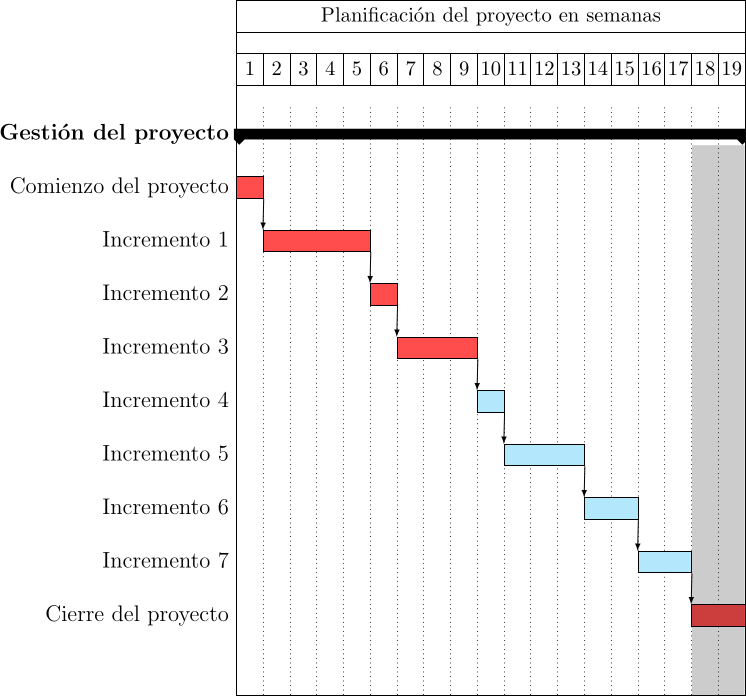
\includegraphics[width=.7\textwidth]{figuras/inicial.png}
	\end{figure}

%Hablar:
	%La idea inicial era presentar en Febrero
\end{frame}

\begin{frame}[fragile]
	\frametitle{Planificación real}

	\begin{figure}[H]
		\centering
		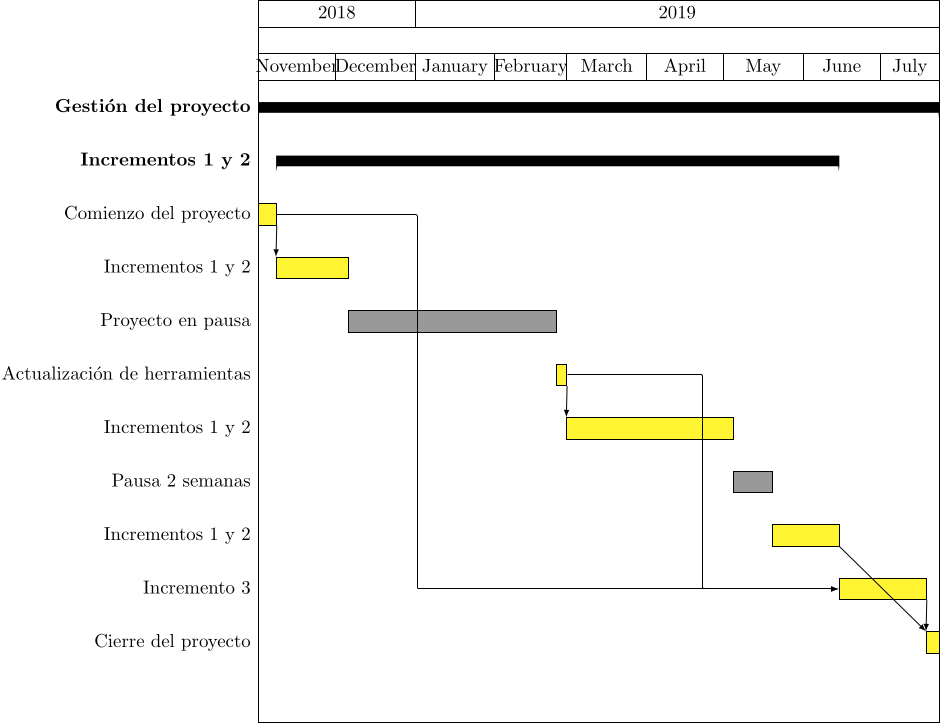
\includegraphics[width=.8\textwidth]{figuras/final.png}
	\end{figure}

%Hablar:
	%Básicamente el incremento 1 se alargó y hubo varias pausas
\end{frame}

\begin{frame}[fragile]
	\frametitle{Laboratorio}

	\begin{figure}[H]
		\centering
		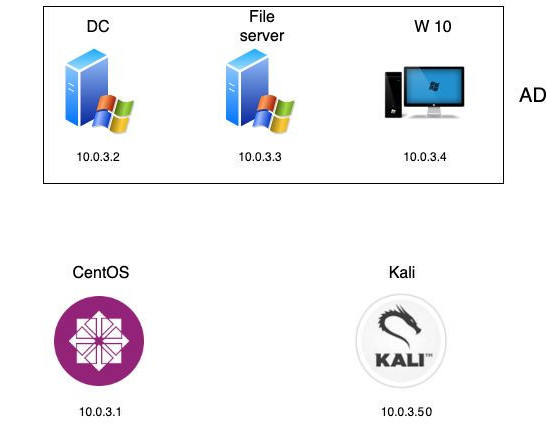
\includegraphics[width=.8\textwidth]{../figuras/virtual_machines.jpg}
	\end{figure}
\end{frame}

\begin{frame}[fragile]
	\frametitle{Gestión de la configuración}

	\begin{itemize}
		\item Identificación y control de los elementos de configuración. %sin versiones, solamente archivado
		\item Git: Código y documentación.
		\item Backups locales: Máquinas virtuales.
	\end{itemize}
\end{frame}


\begin{frame}[fragile]
	\frametitle{Estimación de costes}

\begin{center}
	\begin{tikzpicture}
	\pie [text=legend, color={blue!50, gray!60, yellow!60}, polar, explode=0.1, radius=4] {
		80/RRHH,
		17/Costes indirectos,
		3/Hardware
		%rhh=4897.97
		%hardware=162.39
		%indirectos=1012.07
	}
\end{tikzpicture}
\linej
Total: 6072.43\euro{}
\end{center}

\end{frame}


\begin{frame}[fragile]
	\frametitle{Estimación de costes: RRHH}

	\begin{figure}[H]
		\centering
		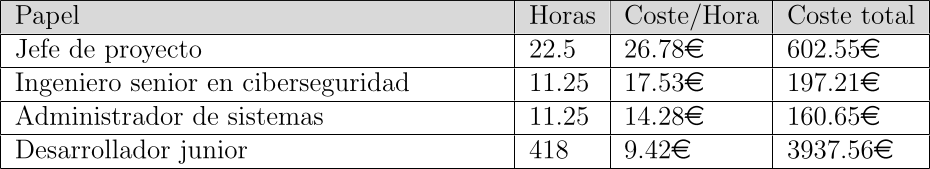
\includegraphics[width=.8\textwidth]{figuras/rrhh.png}
	\end{figure}
\end{frame}

\section{Tecnologías y herramientas}
\begin{frame}[fragile]
	\frametitle{Desarrollo y configuración principal}

	\begin{figure}[H]
		\centering
		
\includegraphics[width=\textwidth]{figuras/TH_principal.png}
	\end{figure}
\end{frame}

\begin{frame}[fragile]
	\frametitle{Pentesting}

	\begin{figure}[H]
		\centering
		
\includegraphics[width=\textwidth]{figuras/TH_pentesting.png}
	\end{figure}
\end{frame}

\begin{frame}[fragile]
	\frametitle{Documentación}

	\begin{figure}[H]
		\centering
		
\includegraphics[width=\textwidth]{figuras/TH_documentacion.png}
	\end{figure}
\end{frame}

\section{Modelo de trabajo}
\begin{frame}[fragile]
	\frametitle{Modelo de trabajo}

	\begin{enumerate}
		\item Análisis del ataque. %dejar claro que es solo para tener la mejor defensa posible
		\item Automatización. %normalmente con varias variantes
		\item Detección. %la detección sin falsos positivos se considera equivalente a una prueba tradicional correcta
	\end{enumerate}
\end{frame}

\section{Incrementos 1 y 2}
\begin{frame}[fragile]
	\frametitle{Golden Ticket}

	\begin{figure}[H]
		\centering
		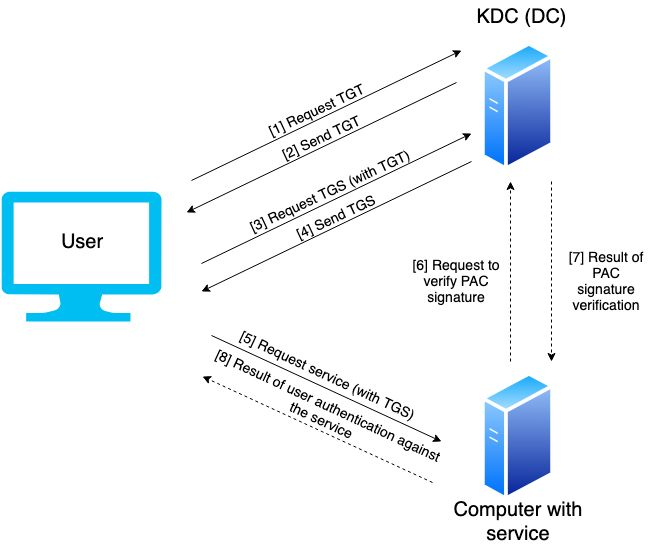
\includegraphics[width=.8\textwidth]{../figuras/TGT_TGS_PAC.jpg}
	\end{figure}

	%La imagen es el esquema de autenticación de Kerberos en Windows
	%Explicar que es el TGT (Ticket Granting Ticket), que sirve para pedir TGSs (tickets para servicios)
	%Puedes poner el usuario que quieras
	%Para generarlo solamente hace falta el hash de la contraseña de la cuenta KRBTGT (superadministrador del KDC [Key Distribution Center]), que se usa para cifrar el ticket
\end{frame}

\begin{frame}[fragile]
	\frametitle{Golden Ticket}

	\begin{itemize}
		\item TGT normal $\xrightarrow{}$ Indetectable. %Además se puede generar offline en otro ordenador
		\item Ticket válido hasta:
		\begin{itemize}
			\item Cambio de contraseña de KRBTGT. %La contraseña del usuario impersonado da igual
			\item Expiración del ticket.
		\end{itemize}
	\end{itemize}
\end{frame}

\begin{frame}[fragile]
	\frametitle{Golden Ticket: Detección}

	\begin{itemize}
		\item Programas usados. %está bien comprobarlo, pero no se puede depender de eso
		\begin{itemize}
			\item Técnicas. %detección especializada para cada caso
			\item DLLs. %sysmon + reglas compuestas
			\item Patrones de texto. %sysmon + reglas atómicas
		\end{itemize}
		\linej
		\item Uso del ticket. %Script klist periódico.
		\begin{itemize}
			\item Usuario raro.
			\item Longevidad. %si el atacante no es precavido va a sobrepasar los 10 minutos por defecto que lo pueden identificar.
		\end{itemize}
	\end{itemize}
\end{frame}

\begin{frame}[fragile]
	\frametitle{Silver Ticket}

	\begin{figure}[H]
		\centering
		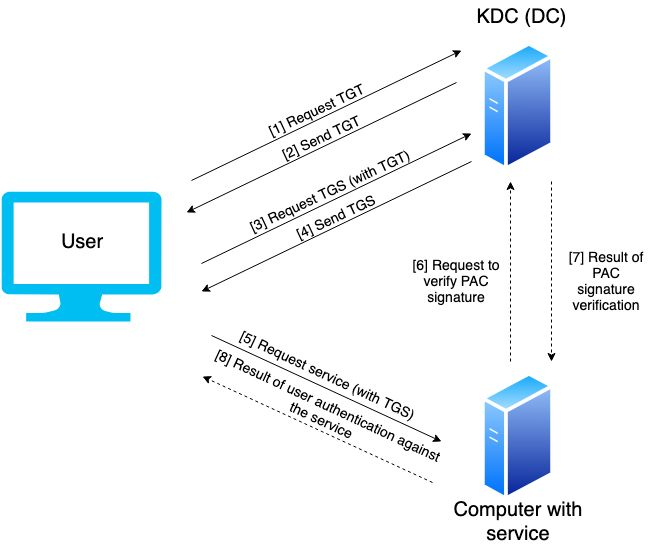
\includegraphics[width=.8\textwidth]{../figuras/TGT_TGS_PAC.jpg}
	\end{figure}

	%Señalar qué es el TGS (paso 5)
	%pueden hacer falta varios TGS para un servicio
	%el TGS está cifrado con el hash de la contraseña del usuario ejecutando el servicio
	%Se detecta de la misma forma que el Golden Ticket
\end{frame}

\begin{frame}[fragile]
	\frametitle{Extracción de credenciales}

	\begin{itemize}
		\item Acceso a archivos clave.
		\item Volcado de memoria.
	\end{itemize}
\end{frame}

%\begin{frame}[fragile]
	%\frametitle{Extracción de credenciales: Detección}

	%\begin{itemize}
		%\item Programas usados. %está bien comprobarlo, pero no se puede depender de eso
		%\begin{itemize}
			%\item Técnicas.
			%\item DLLs.
			%\item Patrones de texto.
		%\end{itemize}
	%\end{itemize}
%Básicamente lo mismo de antes
%\end{frame}

\begin{frame}[fragile]
	\frametitle{PowerShell}

	\begin{itemize}
		\item Ejecución codificada. %se tiene que descodificar en el receptor. Todas las técnicas de detección siguen funcionando.
		\item PowerShell sin \textit{powershell.exe}. %EXE custom, DLLs del sistema
		\begin{itemize}
			\item Ejecución encriptada. %PowerShell v5 puede loggear la ejecución cuando se reconstruye
		\end{itemize}
	\end{itemize}
\end{frame}

\begin{frame}[fragile]
	\frametitle{Logins sospechosos} %trivial

	\begin{itemize}
		\item Fuerza bruta. 				%Misma IP, varias cuentas
		\item Fuerza bruta distribuida. 	%Diferentes IPs, varias cuentas
		\item Fuera de horas normales. 		%script PowerShell periódico
	\end{itemize}
\end{frame}

\section{Incremento 3: Ransomware}
\begin{frame}[fragile]
	\frametitle{Ransomware}

	\begin{itemize}
		\item Recurso como rehén. %el atacante pide rescate
		\item Pago anónimo. %hoy en día es fácil para el atacante recibir dinero sin que sea identificado
		\item Mercado negro. %explicar Ransomware como servicio
		\item Popularidad reciente. %afectando activamente a varios sectores como sanidad o bancos
	\end{itemize}
\end{frame}

\begin{frame}[fragile]
	\frametitle{Crypto ransomware: defensa}

	\begin{itemize}
		\item Detección lo antes posible.
		\begin{itemize}
			\item Encriptación masiva de archivos. %Con Windows Defender, Sysmon, Windows File Auditing, monitorización de integridad de archivos con Wazuh
			\item Borrado de backups. %depende del sistema, pero generalmente el programa intenta borrar por lo menos las de Windows
		\end{itemize}
		\item Respuesta activa. %deseable, pero probablemente insuficiente
		\begin{itemize}
			\item Matarlo.
			\item Apagar.
			\item Desconectar de la red.
			\item Bloquear acceso a los archivos.
		\end{itemize}
		\item Dharma.
	\end{itemize}
\end{frame}

\section{Conclusiones}
\begin{frame}[fragile]
	\frametitle{Conclusiones}

	\begin{itemize}
		\item Mejora de seguridad con Wazuh sin necesidad de conocimiento experto. %cualquiera (más o menos) puede hacer reglas simples, y casi nadie puede hacerlas complejas
		\item Mejor estado de GNU/Linux que Windows para Wazuh. %que necesita muchos workarounds actualmente
		\item Cumplidos los requisitos esenciales, con mucho detalle. %lo he considerado más productivo que los requisitos deseados u opcionales restantes
		\item Tanto IDSs como antivirus tienen sus ventajas y desventajas.
	\end{itemize}
\end{frame}

\begin{frame}[fragile]
	\frametitle{Trabajo futuro}

	\begin{itemize}
		\item Mejoras a Wazuh/OSSEC:
		\begin{itemize}
			\item Creación de reglas. %variables de verdad (sin afectar al rendimiento), reglas composite con freq=1
			\item BDD temporal. %nativa obviamente, para más que IPs
			\item Active response. %más funcionalidad nativa, menos scripts para lo mismo
		\end{itemize}
		\item Incrementos no realizados.
		\item Límites alcance.
	\end{itemize}
\end{frame}



\begin{frame}[fragile]
	\linej
	\linej
	\linej
	\large
	\centerline{\textbf{Mejoras en IDS: añadiendo funcionalidad a Wazuh}}
	\normalsize
	\linej
	\linej
	\centerline{github.com/andresgomezvidal/tfg\_memoria}
	\linej
	\linej
	\begin{multicols}{2}
	\textbf{Autor:}
	\linej
		Andrés Santiago Gómez Vidal
	\linej
	\columnbreak
	\linej
	\textbf{Tutores:}
	\linej
		Purificación Cariñena Amigo
	\linej
		Andrés Tarascó Acuña
	\end{multicols}
\end{frame}





\end{document}
